\documentclass[11pt]{article}
\usepackage[margin=1in]{geometry}
\usepackage{graphicx}
\usepackage{amsmath,amssymb}
\usepackage{booktabs}
\usepackage{natbib}
\usepackage{hyperref}
\usepackage{xcolor}
\usepackage{authblk}
\hypersetup{colorlinks=true, linkcolor=blue!50!black, citecolor=blue!50!black, urlcolor=blue!50!black}

\title{Specific Corticothalamic Connectivity Optimizes Biologically
Plausible Learning in Thalamocortical Loops}
\date{}

\begin{document}
\maketitle

\begin{abstract}
Cortico-thalamo-cortical (CTC) loops are recurrent circuits in which a
small thalamic population exchanges compressed projections with a much
larger cortical population. Recent evidence implicates these loops in a
wide range of motor and cognitive functions, but the computational role
of their specific structure is unclear and, critically, it is not known
whether the connectivity can be acquired through biologically plausible
plasticity. We investigate this question with a recurrent network model
of $N = 256$ cortical neurons reciprocally connected to $M$ uncoupled
thalamic neurons. Thalamocortical synapses are updated by a local
three-factor rule (Random-Feedback-Local-Online, RFLO), while
corticothalamic synapses are either optimized on a slow timescale by
meta-learning or set to idealized subspace-aligned structures. We find
that local plasticity succeeds at thalamocortical synapses but fails at
corticothalamic synapses, because feedback alignment does not propagate
through the thalamic bottleneck. The corticothalamic structure that
supports learning is instead task-specific: readout-aligned
projections, functionally analogous to an efference copy of the motor
command, optimize autonomous motor control, while projections aligned
with the leading principal components of cortical activity optimize
working memory. Meta-learned corticothalamic weights reduce task
error by a median factor of 5.8 for autonomous motor control and 5.1
for working memory relative to random projections, and converge to
precisely these task-specific structures. Reanalysis of recordings from mice grasping (3 sessions, 101
thalamic neurons) and performing delayed discrimination (5 sessions,
72 thalamic neurons) shows that the top 5 cortical principal
components capture a fraction $0.29 \pm 0.02$ of explainable thalamic
variance in motor control but $0.63 \pm 0.04$ in working memory,
matching the model prediction. These results link the anatomy of CTC
loops to computation through the structure of corticothalamic
connectivity.
\end{abstract}

\section{Introduction}

Higher-order thalamic nuclei were for decades treated as passive relays
of sensory and cortical signals, but a growing body of work has
recast them as active participants in cognition and motor control
\cite{sherman2007thalamic, sherman2016thalamus,
halassa2019thalamocortical}. Unlike primary sensory thalamic nuclei,
higher-order nuclei receive the bulk of their driving input from cortex
itself, forming reciprocal cortico-thalamo-cortical (CTC) loops that
have been mapped in rodent sensory, motor, and prefrontal regions
\cite{yamawaki2015synaptic, economo2018distinct, collins2018reciprocal,
guo2018anterolateral}. Perturbation studies in mice demonstrate that
these loops are required for the maintenance of persistent activity
during working memory \cite{guo2017maintenance, bolkan2017thalamic,
schmitt2017thalamic}, for the execution of dexterous movements
\cite{sauerbrei2020cortical}, and for flexible switching among cortical
representations \cite{rikhye2018thalamic, alcaraz2018thalamocortical}.

The computational puzzle raised by this anatomy is that thalamic
populations are much smaller than the cortical populations with which
they interact. A CTC loop therefore implements a compression of cortical
activity into a low-dimensional thalamic space, followed by an expansion
back to cortex. For purely feedforward architectures, theories of
compressed sensing and efficient coding clarify how such bottlenecks
should be structured to preserve or emphasize behaviorally relevant
signals \cite{ganguli2012compressed, olshausen1996emergence}. Recurrent
CTC loops, however, are not feedforward, and insights obtained in
feedforward settings do not transfer directly. Existing theoretical
treatments tune the weights of the loop by numerical optimization and
show that the resulting circuit can support motor preparation or
flexible motor sequencing \cite{kao2021optimal, logiaco2021thalamic}.
What these models do not address is how such tuned weights could be
established by a biologically plausible mechanism.

The question becomes especially pointed when we ask how local,
error-driven plasticity could operate inside a CTC loop. Three-factor
and random-feedback rules have been proposed as biologically plausible
approximations to gradient-based learning in recurrent networks
\cite{murray2019local, lillicrap2016random, gilra2017predicting,
miconi2017biologically, gerstner2018eligibility}, and experimental work
supports plasticity at thalamocortical synapses into adulthood
\cite{hasegawa2018thalamocortical}. Evidence for plasticity at
corticothalamic synapses, however, is limited, and these synapses are
two steps removed from the readout, so that any local learning rule
must contend with a particularly severe credit-assignment problem. We
hypothesized that the ability of the thalamus to contribute to learning
therefore depends on the \emph{structure} of corticothalamic projections
rather than on local plasticity at those projections, and asked what
structure is optimal for which task.

We address this question with a recurrent thalamocortical model in
which $N$ cortical neurons are reciprocally connected to $M$ uncoupled
thalamic neurons with $M \ll N$. Thalamocortical weights are updated by
a local three-factor rule \cite{murray2019local, lillicrap2016random},
while corticothalamic weights are optimized either by meta-learning on
a slow outer-loop timescale \cite{wang2018prefrontal,
hospedales2022meta} or by idealized alignment with specific cortical
subspaces. Our central finding is that the optimal corticothalamic
structure is strongly task-dependent: autonomous motor control benefits
most from a projection carrying an efference copy of the readout, while
working memory benefits most from a projection carrying the leading
principal components of cortical activity. Reanalysis of intracortical
and thalamic recordings from mice performing grasping and
delayed-discrimination tasks \cite{sauerbrei2020cortical,
guo2017maintenance} is consistent with these predictions.

Our contributions are fourfold. First, we show that a local three-factor
plasticity rule succeeds at thalamocortical synapses but fails at
corticothalamic synapses, because feedback alignment does not propagate
through the thalamic bottleneck. Second, we demonstrate that
meta-learning identifies task-specific corticothalamic structures that
reduce task error by a median factor of 5.8 for motor control and 5.1
for working memory relative to random projections. Third, we show that
idealized readout-aligned projections are optimal for motor control
while principal-component-aligned projections are optimal for working
memory, and that these principles generalize to a composite delayed
reaching task in a model with separate preparatory and execution
thalamic modules. Fourth, we reanalyze published neural recordings and
show that the cortical subspaces captured by thalamus in motor cortex
and anterior lateral motor cortex (ALM) match the task-specific
structures predicted by the model.

\section{Related Work}

\paragraph{Higher-order thalamus and cortico-thalamo-cortical loops.}
Reciprocal CTC loops are a frequent anatomical motif across rodent
cortical areas \cite{yamawaki2015synaptic, economo2018distinct,
collins2018reciprocal, guo2018anterolateral,
halassa2019thalamocortical}. Inactivation and optogenetic experiments
show that these loops are required for the maintenance of persistent
activity during working memory and for the execution of prepared
movements \cite{guo2017maintenance, bolkan2017thalamic, schmitt2017thalamic,
sauerbrei2020cortical, rikhye2018thalamic, alcaraz2018thalamocortical}.
Theoretical models have shown that tuned CTC weights can support motor
preparation and flexible motor sequencing \cite{kao2021optimal,
logiaco2021thalamic}, but they rely on numerical optimization and do
not specify a biological mechanism for acquiring the weights. Our work
fills this gap by supplying structured corticothalamic connectivity
together with a local plasticity rule that together realize
biologically plausible learning.

\paragraph{Biologically plausible learning in recurrent networks.}
Classical recurrent learning is non-local \cite{williams1989learning}.
To recover locality, a number of approximations have been introduced:
random feedback alignment \cite{lillicrap2016random}, three-factor
eligibility rules \cite{gerstner2018eligibility, bittner2017behavioral},
dendritic segregation for deep credit assignment
\cite{guerguiev2017towards}, stable local learning in spiking recurrent
networks \cite{gilra2017predicting}, biologically plausible recurrent
network training that reproduces task dynamics
\cite{miconi2017biologically}, and the Random-Feedback-Local-Online
(RFLO) rule that we use here \cite{murray2019local}. These rules have
been analyzed for synapses that directly drive the readout; our results
address the less-studied regime of synapses that are two steps removed
from the readout through the thalamic bottleneck.

\paragraph{Low-rank recurrent network theory and meta-learning.}
Recent theoretical work conceptualizes recurrent connectivity as the sum
of a random full-rank component and a tunable low-rank perturbation
\cite{mastrogiuseppe2018linking}. Because the CTC loop contributes a
rank-$M$ perturbation to the effective cortical connectivity, our
analysis inherits these tools. We combine this framework with
meta-learning \cite{wang2018prefrontal, hospedales2022meta}: a slow
outer loop optimizes the corticothalamic weights, while a fast inner
loop uses a local plasticity rule to update thalamocortical weights.
This two-timescale decomposition is consistent with the view that
corticothalamic structure reflects evolutionary or developmental
processes, while thalamocortical synapses remain plastic throughout
life.

\paragraph{Cortical dynamics during motor learning and cognition.}
Recurrent dynamics have been shown to support flexible computation in
prefrontal cortex and to reorganize during motor learning in rodent
motor cortex \cite{mante2013context, peters2014emergence,
churchland2012neural}. These studies largely attribute learning-induced
changes to plasticity within cortex; our results argue that at least
some of the learning signal is routed through thalamus, and that the
ability of the thalamus to participate depends on the specific
structure of corticothalamic projections.

\section{Methods}

\subsection{Thalamocortical network model}

We consider a network of $N$ recurrently connected cortical neurons
reciprocally coupled to a population of $M$ uncoupled thalamic neurons,
with $M \ll N$ (Figure~\ref{fig:schematic}). We denote cortical
population activity by $h_t \in \mathbb{R}^N$, thalamic population
activity by $r_t \in \mathbb{R}^M$, and external inputs (if any) by
$x_t \in \mathbb{R}^S$. Cortical dynamics evolve as
\begin{equation}
\tau \frac{d h_t}{d t} = -h_t + \phi\!\left(W_{CC} h_t + W_{CT} r_t + W_I x_t \right),
\end{equation}
where $\tau$ is the neuronal time constant and $\phi(\cdot)$ is the
$\tanh$ nonlinearity. The matrices $W_{CC}\in \mathbb{R}^{N\times N}$,
$W_{CT}\in \mathbb{R}^{N\times M}$, and $W_I\in \mathbb{R}^{N\times S}$
denote corticocortical, thalamocortical, and input weight matrices,
respectively. Thalamic activity depends only on cortical activity:
$r_t = \phi(W_{TC} h_t)$, with corticothalamic weights $W_{TC}\in
\mathbb{R}^{M\times N}$. The network output is a linear readout of
cortical activity, $y_t = W_o h_t$, with readout weights $W_o \in
\mathbb{R}^{R\times N}$.

Cortical neurons therefore interact directly via $W_{CC}$ and
indirectly via the thalamic bottleneck, which first compresses
activity into an $M$-dimensional space through $W_{TC}$ and then
expands it back to $N$ dimensions through $W_{CT}$. The effective
interaction matrix can be written as
$W_{\text{eff}} = W_{CC} + W_{CT} V W_{TC}$,
where $V = \mathrm{diag}(\phi'(v_t))$ and $v_t = W_{TC} h_t$ is the
thalamic membrane potential. This effective interaction is thus a
low-rank, rank-$M$ perturbation of the cortical connectivity $W_{CC}$,
consistent with recent work on low-rank recurrent networks
\cite{mastrogiuseppe2018linking}. Unless stated otherwise we use
$N = 256$ and vary $M$ from 1 to 128. In the meta-learning experiments
we use $M = 32$.

\subsection{Local plasticity rule for thalamocortical synapses}

Thalamocortical synapses $W_{CT}$ are adjusted to minimize
$\sum_t \|\varepsilon_t\|^2$, where $\varepsilon_t$ is the mismatch
between the network output $y_t$ and a target function. The weight
updates are derived by applying two approximations to exact
gradient-based recurrent learning \cite{williams1989learning}. First,
nonlocal terms are dropped so that the update to a given
thalamocortical synapse depends only on presynaptic (thalamic) and
postsynaptic (cortical) activities, not on the full state of the
cortex. Second, the error signal is projected back into cortex through
a \emph{random} feedback pathway with weights $B \in \mathbb{R}^{N
\times R}$ rather than the true transpose of the readout
\cite{lillicrap2016random}. The readout weights $W_o$ are co-adapted
by a delta rule so that alignment between $B^T$ and $W_o$ emerges over
learning. The resulting update for thalamocortical synapses is of the
three-factor form \cite{murray2019local, gerstner2018eligibility},
\begin{equation}
\Delta W_{CT}^{ij} \propto \left(B \varepsilon_t\right)_i \, p_{ij},
\qquad
p_{ij} \leftarrow \left(1 - \tfrac{1}{\tau_p}\right) p_{ij} + \tfrac{1}{\tau_p} \phi'(u_i) \, r_j,
\end{equation}
where $(B \varepsilon_t)_i$ is the error signal projected onto cortical
neuron $i$, $u_i$ is its membrane potential, $r_j$ is the presynaptic
thalamic activity, and $p_{ij}$ is an eligibility trace storing the
recent correlation between thalamic unit $j$ and cortical unit $i$.
The readout is updated by a standard delta rule,
$\Delta W_o^{ki} \propto \varepsilon_k(t)\, h_i(t)$, where
$\varepsilon_k(t)$ is the error in the $k$-th output dimension.

\subsection{Meta-learning of corticothalamic weights}

Since local plasticity cannot optimize $W_{TC}$ in a biologically
plausible way (Section~\ref{sec:local}), we treat $W_{TC}$ as a slow
variable set by evolutionary or developmental processes
\cite{wang2018prefrontal, hospedales2022meta}. We optimize $W_{TC}$ via
a meta-learning procedure: an \emph{outer loop} optimizes $W_{TC}$
across thousands of epochs, each of which comprises an \emph{inner
loop} of a few hundred trials of thalamocortical learning with the
local rule above. At the start of each outer-loop epoch, $W_{CT}$ is
reset so that the corticothalamic weights discovered by the outer loop
do not depend on the initial state of $W_{CT}$. During meta-learning we
fix all other weights and enforce feedback alignment $B^T = W_o$; we
relax these constraints later and verify that the conclusions hold.
Optimization of $W_{TC}$ is performed by backpropagation through time.
Once $W_{TC}$ is fixed, we measure task performance by training
$W_{CT}$ with the local rule and computing the $R^2$ between the
network output and the target.

\subsection{Idealized subspace-aligned corticothalamic connectivity}

To test which cortical subspaces are individually sufficient for
thalamocortical learning, we consider three idealized forms of
$W_{TC}$ with increasing structure: (i) a random $M$-dimensional
subspace of cortical activity; (ii) $W_{TC}$ aligned with the leading
$M$ principal components of cortical activity, so that each thalamic
neuron receives one of the top-$M$ PCs; and (iii) $W_{TC}$ aligned with
the readout direction $W_o$ and thus carrying a copy of the network
output to thalamus. We quantify alignment $\beta$ between $W_{TC}$ and
a given cortical direction in a normalized scale
$(\beta - \beta_0)/(1 - \beta_0)$, where $\beta_0$ is the average
alignment between the meta-learned $W_{TC}$ and a random direction in
cortical activity space.

\subsection{Tasks}

We study three tasks. The \emph{autonomous motor control} task requires
the network to output a complex temporal waveform without external
inputs during the output phase, analogous to the EMG activity needed
for internally generated movement. The \emph{working memory} task
requires the network to output the amplitude of one of eight possible
transient input pulses during a subsequent delay period. The
\emph{delayed reaching} task combines both computations: the model
must execute a reaching movement to a transiently cued location on a
two-dimensional screen, with movement initiated only after a go cue
that arrives following a random delay. The reaching model uses two
thalamic nuclei (preparatory and execution) with $M = 2$ each, and the
network output drives the angular accelerations of a two-joint arm.
Task complexity is varied either by scaling the frequency of the
target waveform (motor control) or by increasing the number of unique
input amplitudes to be memorized (working memory).

\subsection{Analysis of neural recordings}

We reanalyzed published datasets of simultaneous cortical and thalamic
recordings from mice performing a reach-to-grasp motor control task
(motor cortex and motor thalamus) \cite{sauerbrei2020cortical} and a
delayed discrimination working-memory task (ALM and VM/VAL thalamus)
\cite{guo2017maintenance}. We used a linear regression model to decode
behavior (hand acceleration in motor control; choice in working
memory) and the activity of individual thalamic neurons from the
cortical population activity. This analysis estimates which modes of
cortical activity propagate to behavior (readout weights $W_o$) and to
thalamus (corticothalamic weights $W_{TC}$). Analyses were restricted
to the movement period in motor control and the delay period in
working memory. To compute the contribution of the top $k$ cortical
principal components we decoded thalamic activity using only those
components. We report the fraction of explainable variance as
$R^2(k)/R^2$, where $R^2$ uses the full cortical population. To test
whether corticothalamic interactions reflect genuine cortex-to-thalamus
coupling rather than common inputs, we compared predictions of thalamic
activity using simultaneously recorded cortical activity (within-trial)
against trial-averaged cortical predictions and against shuffled trial
indices as a chance baseline.

\section{Results}

\subsection{Local plasticity succeeds for thalamocortical but fails for corticothalamic synapses}
\label{sec:local}

Credit assignment inside a CTC loop has two qualitatively different
pieces: synapses $W_{CT}$ from thalamus onto cortex are one step from
the readout, while synapses $W_{TC}$ from cortex onto thalamus are two
steps away, with cortical dynamics and $W_{CT}$ interposed between
them and the behavioral output. We first asked whether a single local
plasticity rule could update both. We applied the RFLO-style update
rule to $W_{CT}$ alone, $W_{TC}$ alone, or both simultaneously,
varying the thalamic population size $M$ from 1 to 128 while holding
$N = 256$. Updating $W_{CT}$ with the local rule
progressively improved performance as $M$ increased, consistent with
thalamocortical plasticity facilitating learning. In contrast,
applying an analogous rule to $W_{TC}$ failed to yield improvement
even when the thalamic population was comparable in size to the
cortex. Updating both sets of synapses simultaneously was no better
than updating only $W_{CT}$, indicating that the extra plasticity on
the corticothalamic side did not contribute.

The failure is understandable from the credit-assignment structure of
the loop. Corticothalamic synapses are upstream of the readout in the
sense that updating them changes thalamic membrane potentials, which
in turn reshape cortical dynamics only through the subsequent action
of $W_{CT}$. A local rule at $W_{TC}$ therefore requires error signals
gated through both the time-varying cortical state and the current
$W_{CT}$, which cannot be easily delivered to a thalamic neuron by
local quantities. Consistent with this interpretation, feedback
alignment between the random feedback matrix $B$ and the readout
$W_o$ reached above-chance levels in cortical neurons but not in
thalamic neurons under the local rule. These observations suggest that
error-driven plasticity alone is insufficient to set corticothalamic
connectivity. If corticothalamic structure cannot be learned online
from behavioral error, then some slower optimization process must
supply it, which motivates the meta-learning approach we take next.

\subsection{Meta-learning identifies task-specific corticothalamic structure}

If local plasticity cannot optimize $W_{TC}$, another mechanism --
most plausibly evolution or development -- must select corticothalamic
connectivity. We formalized this with a meta-learning procedure in
which $W_{TC}$ was optimized on a slow outer-loop timescale, while the
inner loop trained $W_{CT}$ with the local rule from scratch on each
epoch (Figure~\ref{fig:schematic}). All models had $N = 256$ cortical
neurons and $M = 32$ thalamic neurons
\cite{wang2018prefrontal, hospedales2022meta}.

Meta-learning substantially improved performance in both tasks. The
task error $1 - R^2$ fell several fold when $W_{TC}$ was
meta-learned relative to a random baseline: the median factor of
error reduction was 5.8 for motor control and 5.1 for working memory
(Figure~\ref{fig:meta_gain}). The improvement was robust to random
error feedback during learning, ruling out the concern that
meta-learning was exploiting feedback alignment enforced during the
outer loop. Equivalent gains were obtained whether or not $W_{TC}$ was
pre-aligned with the readout at the start of meta-learning.

To understand what structure the outer loop had discovered, we
computed the alignment between the meta-learned $W_{TC}$ and two
natural cortical directions: the readout direction $W_o$ and the
leading principal component of cortical activity. In motor control,
the meta-learned $W_{TC}$ was significantly more aligned with the
readout than with the leading principal component. In working memory,
the pattern reversed: the meta-learned $W_{TC}$ was more strongly
aligned with the leading principal component. Thus the outer-loop
optimization converged to qualitatively different corticothalamic
structures depending on the task, pointing to a nontrivial interplay
between corticothalamic structure and task demands.

\subsection{Idealized subspace-aligned corticothalamic connectivity}

The meta-learning results suggested that specific cortical subspaces
carry the signal that supports thalamocortical learning. To test this
idea directly, we constructed three idealized models of
corticothalamic connectivity and trained $W_{CT}$ with the local rule
in each. We began in the most compressed regime, $M = 1$, where only a
one-dimensional subspace of cortical activity is available.

With $M = 1$, learning was possible only when the single
corticothalamic projection was aligned with the right subspace. For
autonomous motor control, readout alignment yielded substantially
better performance than either a random or PC-aligned projection; the
median $-\log(1 - R^2)$ was 1.2 for random $W_{TC}$, 1.2 for
PC-aligned $W_{TC}$, and 2.1 for readout-aligned $W_{TC}$
(Figure~\ref{fig:idealized_m1}). For working memory, the relationship
was inverted: the PC-aligned projection was best, with values of 1.9,
2.5, and 1.8 for random, PC-aligned, and readout-aligned $W_{TC}$,
respectively. Random corticothalamic connectivity learned poorly in
both tasks, even on the simplest variants we tested.

These conclusions held at higher $M$. As the thalamic population size
was increased toward the cortical size, the performance of all three
idealized models gradually improved, because an increasingly larger
subspace of cortical activity was available to support learning.
However, the advantage of readout alignment in motor control and PC
alignment in working memory persisted across a wide range of $M$ and
across a range of task complexities. Thalamocortical learning also
benefited from approximate forms of the structured connectivity: the
readout signal did not need to be concentrated on a single thalamic
neuron for motor control, the PCs did not need to be segregated across
different thalamic neurons for working memory, and structure that
emerged gradually in conjunction with thalamocortical learning was
still useful. We further found that the benefits of subspace-aligned
connectivity were absent when $W_{CT}$ was held fixed, confirming that
the structure of $W_{TC}$ improves task performance specifically by
enabling thalamocortical plasticity and not by merely relaying
behaviorally informative activity.

Why does each task pair with a specific cortical subspace? Examining the
principal components of cortical activity revealed that in the motor
control task the leading PCs fluctuate slowly and therefore cannot
reconstruct the high-frequency components of the target waveform; a
signal aligned with the readout is required. In the working memory
task, by contrast, the leading PCs are dominated by the transient
input pulses and encode stimulus identity; projecting this signal to
the thalamus allows thalamocortical synapses to build the persistent
activity needed to span the delay.

\subsection{Composite task: delayed reaching}

Naturalistic behavior often requires a combination of motor control
and memory, and we therefore asked whether the same structural
principles extend to a composite task. We considered a goal-directed
reaching task in which the model received a transient location cue and
then, following a randomly timed go cue, had to produce torques
driving a two-joint arm to the target. Motivated by reports of
distinct preparatory and execution populations in motor thalamus -- a
dissociation paralleled by the functional segregation of ALM/VM-VAL
\cite{guo2017maintenance} and motor cortex/motor thalamus
\cite{sauerbrei2020cortical} loops used in our data reanalysis -- we
equipped the model with two thalamic nuclei, each of $M = 2$ neurons,
gating in only during the preparatory or only during the execution
phase. Corticothalamic weights onto each nucleus were independently
set to a random, PC-aligned, or readout-aligned structure, and
$W_{CT}$ was trained with the local rule.

Performance was maximized when the preparatory thalamic nucleus
received PC-aligned inputs and the execution nucleus received
readout-aligned inputs -- the combination predicted by the
task-dependent principles identified above. This configuration
produced accurate reaching trajectories to all eight target locations
and was robust to the number of targets and to the distribution of
delays. Thus a single cortex paired with distinct structured thalamic
modules can learn a task whose phases make different computational
demands, consistent with the experimental finding that separate
populations of motor thalamic neurons are active during movement
preparation and movement execution.

\subsection{Neural data from mice are consistent with model predictions}

The model makes two concrete predictions about corticothalamic
interactions in behaving animals: in motor tasks, corticothalamic
weights should align with the readout; in working memory tasks, they
should align with the leading principal components of cortical
activity. We tested both predictions by reanalyzing published
recordings of simultaneous cortical and thalamic activity from mice
performing a reach-to-grasp motor control task (motor cortex and motor
thalamus, 3 sessions, 101 thalamic neurons)
\cite{sauerbrei2020cortical} and a delayed discrimination working
memory task (ALM and VM/VAL thalamus, 5 sessions, 72 thalamic
neurons) \cite{guo2017maintenance}.

Cortical activity was strongly predictive of behavior in both
datasets, with $R^2 = 0.93$ for hand acceleration during the motor
task and $R^2 = 0.97$ for choice during the working memory task
(Figure~\ref{fig:behavior_decoding}). Critically, the cortical
directions carrying this behavioral signal were different in the two
tasks: the leading cortical principal components had a large influence
on the behavioral choice in working memory, whereas hand movements
during the motor task were primarily driven by principal components
of lower variance. This difference in readout structure is consistent
with the model and sets up a test of the corticothalamic prediction.

We next estimated the fraction of variance in each thalamic neuron
that could be explained by cortical activity. Using the full cortical
population, we captured $R^2 = 0.46 \pm 0.01$ of the thalamic variance
during the motor control task and $R^2 = 0.70 \pm 0.01$ during the
working memory task. We then asked how much of this explainable
variance was already captured by the top $k$ cortical principal
components. Because the working memory task is driven by the leading
PCs, the model predicts that a small number of PCs should suffice to
explain thalamic activity; because the motor task relies on
lower-variance readout-aligned directions, the model predicts that
many more PCs should be needed. Exactly this pattern emerged in the
data: the top 5 cortical PCs captured $0.29 \pm 0.02$ of explainable
thalamic variance in motor control and $0.63 \pm 0.04$ in working
memory (Figure~\ref{fig:thalamic_variance}), a striking and
predicted dissociation.

Finally, we asked whether the observed corticothalamic coupling
reflects genuine cortical drive rather than common input. In the
working memory task, cortical inactivation dramatically reduces
thalamic variability \cite{guo2017maintenance}, directly implicating
cortex as a causal driver. Inactivation was not performed in the motor
dataset, but the simultaneity of the cortical and thalamic recordings
allowed an indirect test: trial-by-trial fluctuations in motor cortex
were substantially more predictive of thalamic activity on the same
trial than trial-averaged cortical activity. Furthermore, the
corticothalamic weights that captured trial-by-trial thalamic activity
were more strongly aligned with the readout weights than those
capturing only trial-averaged thalamic activity. This pattern is
consistent with motor thalamus receiving an efference copy of the
motor command from cortex. Taken together, the across-task pattern
observed in the neural data -- high-variance PC alignment in the
working memory loop, lower-variance readout alignment in the motor
loop -- matches the task-specific corticothalamic structures that our
model predicts are required to support biologically plausible
thalamocortical learning.

\subsection{Summary of numerical results}

Table~\ref{tab:metalearning} summarizes the meta-learning gains.
Table~\ref{tab:idealized} reports task performance at maximum
compression for each idealized corticothalamic structure.
Table~\ref{tab:variance} reports the fraction of thalamic variance
captured in the neural recordings, and Table~\ref{tab:behavior}
reports the decoding of behavior from cortical activity.

\begin{table}[htbp]
\centering
\caption{Error reduction from meta-learned vs.\ random corticothalamic
weights. Values are median factors across simulations.}
\label{tab:metalearning}
\begin{tabular}{lc}
\toprule
Task & Median factor of error reduction \\
\midrule
Motor control & 5.8 \\
Working memory & 5.1 \\
\bottomrule
\end{tabular}
\end{table}

\begin{table}[htbp]
\centering
\caption{Performance of idealized corticothalamic connectivity at
maximum compression ($M = 1$), measured as median $-\log(1 - R^2)$
(higher is better) on the two tasks. The best structure for each task
is readout-aligned for motor control (2.1) and PC-aligned for working
memory (2.5).}
\label{tab:idealized}
\begin{tabular}{lcc}
\toprule
Connectivity type & Motor control & Working memory \\
\midrule
Random  & 1.2 & 1.9 \\
PC-aligned & 1.2 & 2.5 \\
Readout-aligned & 2.1 & 1.8 \\
\bottomrule
\end{tabular}
\end{table}

\begin{table}[htbp]
\centering
\caption{Fraction of thalamic variance explained by cortical activity
in the two neural datasets. $R^2_\text{all}$ uses the full cortical
population; $R^2_\text{top5}$ uses only the top 5 cortical principal
components. Values are mean $\pm$ SEM across thalamic neurons.}
\label{tab:variance}
\begin{tabular}{lcc}
\toprule
Task & $R^2_\text{all}$ & $R^2_\text{top5}/R^2_\text{all}$ \\
\midrule
Motor control  & $0.46 \pm 0.01$ & $0.29 \pm 0.02$ \\
Working memory & $0.70 \pm 0.01$ & $0.63 \pm 0.04$ \\
\bottomrule
\end{tabular}
\end{table}

\begin{table}[htbp]
\centering
\caption{Decoding of behavior from cortical population activity, and
dataset sizes.}
\label{tab:behavior}
\begin{tabular}{lccc}
\toprule
Task & $R^2$ (behavior) & Sessions & Thalamic neurons \\
\midrule
Motor control  & 0.93 & 3 & 101 \\
Working memory & 0.97 & 5 & 72 \\
\bottomrule
\end{tabular}
\end{table}

% -- figures --
\begin{figure}[tbp]
\centering

\includegraphics[width=0.75\textwidth]{figures/fig_schematic.pdf}
\caption{\textbf{Thalamocortical loop architecture.} A recurrent
cortical network of $N = 256$ neurons is reciprocally connected to an
uncoupled thalamic population of $M = 32$ neurons via corticothalamic
($W_{TC}$) and thalamocortical ($W_{CT}$) weights. Recurrent cortical
connections ($W_{CC}$) are fixed. The local RFLO plasticity rule
updates thalamocortical weights $W_{CT}$; corticothalamic weights
$W_{TC}$ are either optimized by meta-learning on a slow timescale or
set to an idealized structure aligned with a specific cortical
subspace.}
\label{fig:schematic}
\end{figure}

\begin{figure}[tbp]
\centering
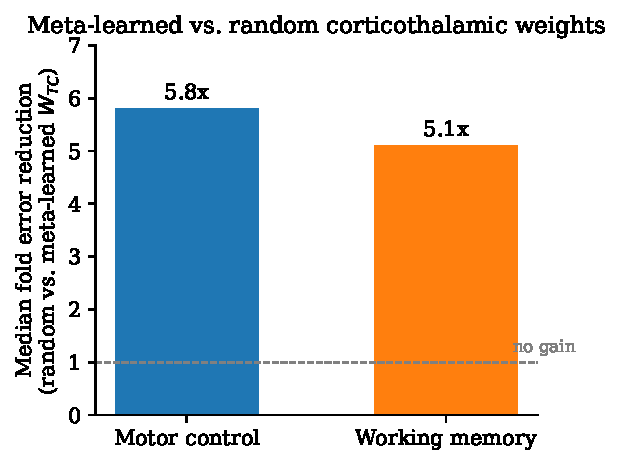
\includegraphics[width=0.62\textwidth]{figures/fig_metalearning_gain.pdf}
\caption{\textbf{Meta-learning reduces task error several fold
relative to random corticothalamic weights.} Median factor by which
task performance error decreases when $W_{TC}$ is meta-learned
compared with the random $W_{TC}$ baseline. Across simulations,
meta-learning yields a 5.8-fold improvement for the autonomous motor
control task and a 5.1-fold improvement for the working memory task.
All models have $N = 256$ cortical neurons and $M = 32$ thalamic
neurons.}
\label{fig:meta_gain}
\end{figure}

\begin{figure}[tbp]
\centering
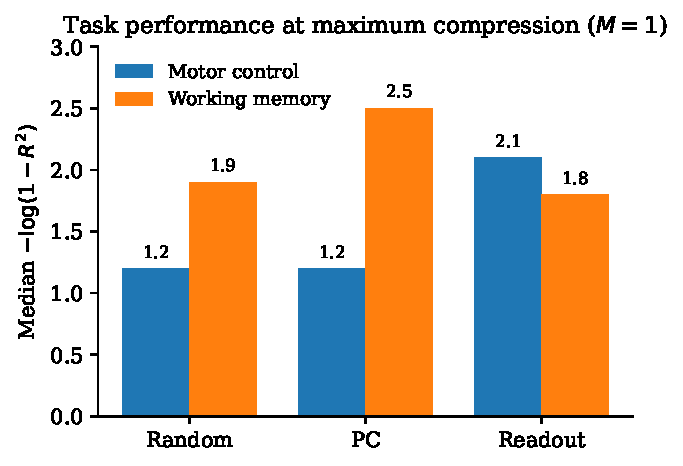
\includegraphics[width=0.72\textwidth]{figures/fig_idealized_m1.pdf}
\caption{\textbf{Idealized corticothalamic connectivity at maximum
compression.} Median $-\log(1 - R^2)$ for models with $M = 1$ and
corticothalamic weights aligned with a random direction, with the
leading principal component direction (PC), or with the readout
direction. Higher values indicate better performance. Motor control is
optimally supported by readout-aligned corticothalamic weights (2.1),
while working memory is optimally supported by PC-aligned weights
(2.5). Random connectivity learns poorly in both tasks (1.2 and 1.9).}
\label{fig:idealized_m1}
\end{figure}

\begin{figure}[tbp]
\centering
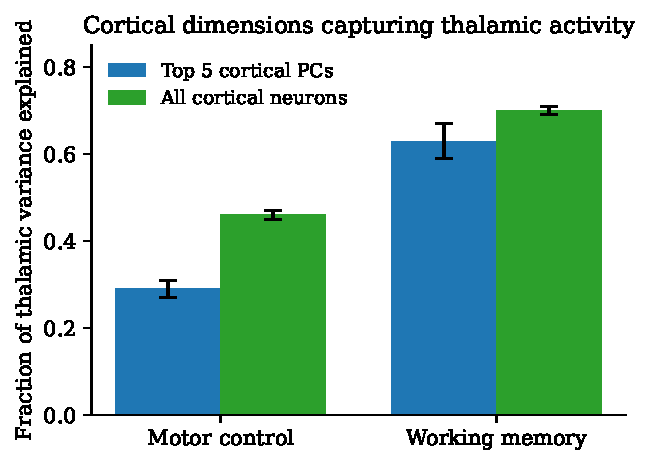
\includegraphics[width=0.72\textwidth]{figures/fig_thalamic_variance.pdf}
\caption{\textbf{Cortical dimensions capturing thalamic activity in
mice.} Fraction of variance in individual thalamic neurons explained
by the top 5 cortical principal components versus by the full cortical
population. The top 5 cortical PCs capture $0.29 \pm 0.02$ of
explainable thalamic variance in motor control but $0.63 \pm 0.04$ in
working memory, consistent with the model prediction that motor
thalamus is driven by lower-variance readout-aligned directions while
frontal thalamus is driven by the leading principal components of
cortical activity. Error bars are $\pm 1$ SEM.}
\label{fig:thalamic_variance}
\end{figure}

\begin{figure}[tbp]
\centering
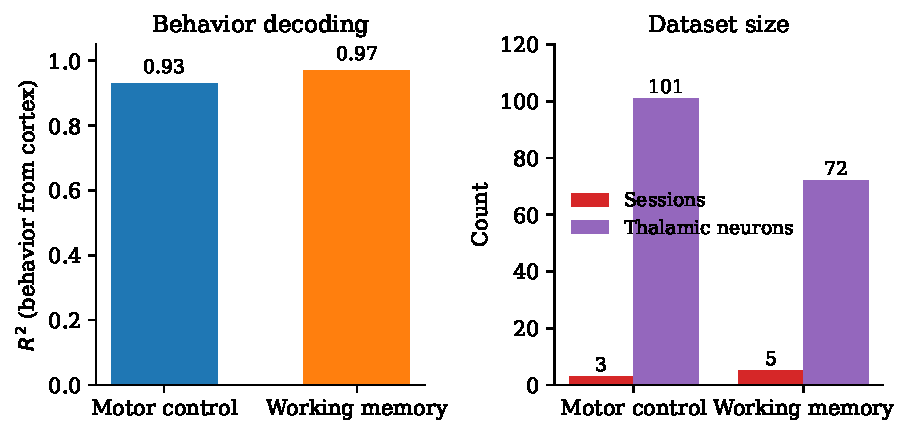
\includegraphics[width=0.85\textwidth]{figures/fig_behavior_decoding.pdf}
\caption{\textbf{Behavior decoding and dataset size for the two
re-analyzed neural recordings.} Left: Fraction of variance in behavior
(hand acceleration for motor control; choice for working memory)
explained by a linear readout of cortical population activity.
Cortical activity explains 0.93 of behavioral variance in motor
control and 0.97 in working memory. Right: Number of recording
sessions and number of thalamic neurons in each dataset. Motor
control: 3 sessions, 101 thalamic neurons (motor cortex and motor
thalamus). Working memory: 5 sessions, 72 thalamic neurons (ALM and
VM/VAL thalamus).}
\label{fig:behavior_decoding}
\end{figure}

\section{Discussion}

The connectivity of cortico-thalamo-cortical loops must be organized
for the loop to contribute to learning, and our analysis shows that
the organizing principle is remarkably simple: the corticothalamic
projection should communicate the cortical subspace that is most useful
for the task being learned. In our model, this principle manifests
as a task-specific structure -- readout alignment for motor control,
principal-component alignment for working memory -- that local
error-driven plasticity cannot discover but that meta-learning, a
proxy for evolutionary or developmental optimization, finds reliably
and that the data appear to respect. These findings connect two ideas
that have largely been pursued in parallel: theories that treat
recurrent networks as the sum of a random matrix and a tunable
low-rank perturbation \cite{mastrogiuseppe2018linking}, and
experimental work showing that thalamocortical plasticity supports
learning in adult animals \cite{hasegawa2018thalamocortical}. They do
so by specifying how the tunable low-rank perturbation contributed by
the CTC loop must be structured if biologically plausible plasticity
\cite{murray2019local, lillicrap2016random, gerstner2018eligibility}
is to succeed.

The conclusion that corticothalamic structure should be efference-copy-like
for motor learning is anatomically plausible. Tracing studies have long
identified an evolutionarily conserved projection from layer V
pyramidal neurons to higher-order thalamus via axonal branching of
corticofugal projections to motor targets \cite{yamawaki2015synaptic,
economo2018distinct}. Since the primary targets of these corticofugal
projections are descending motor pathways, the same branch that carries
motor commands to lower centers is well placed to carry an efference
copy of those commands to thalamus. Our reanalysis of motor cortex
recordings \cite{sauerbrei2020cortical} showed that the alignment of
thalamic activity with the cortical motor output was significantly
greater than chance, and that the alignment became stronger when
predictions used trial-by-trial cortical fluctuations rather than
trial-averaged activity. The alignment we observe is partial rather
than perfect, but partial alignment is already sufficient to produce
the learning gains in our idealized models. One caveat is that we used
limb acceleration as a proxy for motor output, while an EMG-based
proxy would be closer to the theoretical construct; another is that
some corticofugal branches target midbrain rather than spinal cord
\cite{economo2018distinct}, suggesting that only a subset of motor
thalamic loops may participate in this type of learning.

The conclusion that higher-order thalamic projections from frontal
cortex should encode the leading principal components of cortical
activity points toward a different biological mechanism. Leading PCs
can be extracted by unsupervised, Hebbian-like plasticity that does
not require a gated error signal and is therefore available even in
the absence of the specialized feedback machinery needed for
error-driven learning at cortico-thalamic synapses. Our analysis of
delayed discrimination recordings \cite{guo2017maintenance} shows that
a small number of leading cortical PCs suffice to explain most of the
thalamic variance, and optogenetic silencing in that dataset
establishes cortex as a causal driver of thalamic activity. The
pathway from ALM to VM/VAL thalamus
\cite{guo2018anterolateral, collins2018reciprocal} emerges from this
analysis as a strong candidate for investigating Hebbian forms of
plasticity in higher-order thalamus.

Several aspects of our model are deliberately simplified, and the
consequences of relaxing them define a natural set of extensions.
Cortical and thalamic populations here are homogeneous, whereas
biological circuits show rich heterogeneity across cortical layers
\cite{economo2018distinct, guo2018anterolateral}, diversity in
membrane properties across thalamic neurons, and convergence of inputs
from multiple cortical areas onto single thalamic neurons. Our model
uses a single error-driven plasticity rule \cite{murray2019local},
whereas reward-based rules, spike-based rules
\cite{gilra2017predicting}, and dendrite-based credit assignment
\cite{guerguiev2017towards, bittner2017behavioral} are all plausible
substrates for thalamocortical plasticity. We also do not explicitly
model other subcortical drivers of thalamus: the cerebellum and basal
ganglia interact with corticothalamic inputs and could modulate
thalamocortical plasticity in ways our model does not capture, and
local inhibition via the thalamic reticular nucleus is likely to shape
which cortical subspaces arrive at any given thalamic neuron.
Nonetheless, the structural principle we identify is robust to many of
these relaxations, as evidenced by the fact that our composite
reaching model achieved good performance by combining two simple
corticothalamic structures and by the consistent support from the
available neural data.

The two-timescale organization of our model -- slow evolutionary
tuning of $W_{TC}$, fast error-driven tuning of $W_{CT}$ -- also
suggests a plausible substrate for continual and context-dependent
learning. Different CTC loops carry different cortical subspaces to
thalamus, and thalamocortical plasticity in each loop can therefore
learn task components whose signals are routed through that loop
without overwriting components learned through other loops. Subcortical
structures can plausibly gate which loop is engaged in which context:
although we do not explicitly model the basal ganglia, our composite
reaching result, in which distinct thalamic modules were active during
preparatory and execution phases, is in the spirit of a BG-mediated
switching signal that selects the thalamic subsystem best matched to
the current computational demand. The same mechanism could underlie
switching among cortical representations reported for higher-order
thalamus \cite{rikhye2018thalamic, schmitt2017thalamic} and suggests
corticothalamic structure as one axis along which the brain could
mitigate catastrophic interference.

Our results also bear on learning-induced reorganization of cortical
representations \cite{peters2014emergence, mante2013context}. The
prevailing interpretation of such reorganization attributes it to
plasticity at corticocortical synapses. Our model suggests that a
substantial portion of the reorganization could instead reflect
changes at thalamocortical synapses within CTC loops, driven by the
corticothalamic structure we identify. Disentangling the contributions
of thalamocortical and corticocortical plasticity is an important
direction for future studies; one attractive possibility is that
different CTC loops are engaged in different contexts, with
thalamocortical plasticity responsible for context-specific components
and corticocortical plasticity consolidating components shared across
contexts. More broadly, our results argue that understanding the
connectivity of higher-order thalamus is not merely an anatomical
exercise: the specific structure of corticothalamic projections
determines what the thalamus can compute, what can be learned through
it, and how. Establishing that link is, we believe, a necessary step
toward a biologically grounded theory of cortico-thalamo-cortical
function.

\bibliographystyle{plainnat}
\bibliography{references}

\end{document}
